\documentclass[11pt,professionalfonts,aspectratio=169,final]{beamer}

\usepackage{presentation_packages}
%\bibliography{library} % must be in the preamble when using biblatex package

\definecolor{mygray}{gray}{0.9}
\definecolor{RoyalBlue}{rgb}{0.25,0.41,0.88}
\def\Emph{\textcolor{RoyalBlue}}

\definecolor{tmp}{rgb}{0.804,0.941,1.0}
\setbeamercolor{numerical}{fg=black,bg=tmp}
\setbeamercolor{exact}{fg=black,bg=red}

\mode<presentation> 
{
  \usetheme[hideothersubsections,width=3.5\baselineskip]{Berkeley}
  % \usefonttheme{serif}
  \setbeamercovered{transparent}
  \setbeamerfont{section in sidebar}{size=\scriptsize}
  \setbeamerfont{subsection in sidebar}{size=\tiny}
}

\makeatletter
\beamer@headheight=1.5\baselineskip

\setbeamertemplate{sidebar \beamer@sidebarside}%{sidebar theme}
  {
    \beamer@tempdim=\beamer@sidebarwidth%
    \advance\beamer@tempdim by -6pt%
    \insertverticalnavigation{\beamer@sidebarwidth}%
    \vfill
    \ifx\beamer@sidebarside\beamer@lefttext%
    \else%
      \usebeamercolor{normal text}%
      \llap{\usebeamertemplate***{navigation symbols}\hskip0.1cm}%
      \vskip2pt%
    \fi%
}%

\setbeamertemplate{footline}%{split theme}
{%
  \leavevmode%
  \begin{beamercolorbox}[wd=1\paperwidth,ht=2.5ex,dp=1.125ex,leftskip=.3cm,rightskip=.3cm]{title in head/foot}
%    \usebeamerfont{title in head/foot}\mypaper\hfill \insertframenumber/\inserttotalframenumber
    \usebeamerfont{title in head/foot}\insertshorttitle \hfill \insertframenumber/\inserttotalframenumber
  \end{beamercolorbox}
} 
\setbeamertemplate{blocks}[rounded][shadow=true]
\setbeamertemplate{title page}[default][shadow=true,rounded=true]
\setbeamercolor{box}{fg=black,bg=yellow}
\makeatother

\title[Why Python?]{\large\bf  Intro to Scientific Python}

\author[FDCL]{Shankar Kulumani}

%\institute{\footnotesize
%{\normalsize Shankar Kulumani}\vspace*{0.2cm}\\
%  Flight Dynamics and Control Lab \\ 
%  Dept. of Mechanical and Aerospace Engineering\\ 
%  The George Washington University \\
%  Washington, DC\\ \vspace{10pt}
%  June 4, 2014 \\ \vspace{10pt}
%  }
\date{2017 March 3}

\institute{
\large{\textbf{Flight Dynamics \& Control Lab}}\\
  \begin{figure} %figure%
        
\includegraphics[width=0.75\textwidth]{gw_txh_2cs_pos}
    \end{figure}
}

\logo{
\includegraphics[scale=0.2]{figures/gw_atx_2cs_rev.pdf}}

\begin{document}

\setcounter{framenumber}{-1}
\begin{frame} %-----------------------------%
  \titlepage
\end{frame}   %-----------------------------%

\begin{frame}{Get Scientific Python!}
\begin{columns}
\begin{column}{0.5\textwidth}
\begin{itemize}
    \item Python is a general language, but we care about the science!
    \item Easiest way is the \href{https://www.continuum.io/downloads}{Anaconda} distribution
    \item Includes everything we need to for Python and science in a easy to manage package
\end{itemize}
\end{column}
\begin{column}{0.5\textwidth}
    \begin{figure}
        \centering
        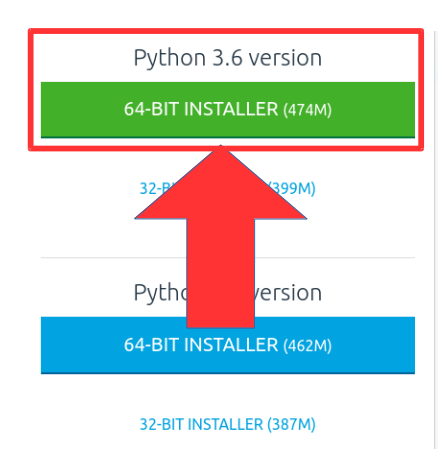
\includegraphics[width=\columnwidth,height=0.8\textheight,keepaspectratio]{figures/anaconda3.png}
        \caption{Just get Python 3}
    \end{figure}
\end{column}
\end{columns}
\end{frame}

\begin{frame}{History of Python}
    \begin{columns}
    \begin{column}{0.5\textwidth}
        \begin{itemize}
            \item \href{https://en.wikipedia.org/wiki/Guido_van_Rossum}{Guido van Rossum} started creating Python in 1989
        \end{itemize}
        \begin{block}{}
        Over six years ago, in December 1989, I was looking for a "hobby" programming project that would keep me occupied during the week around Christmas. \ldots I chose Python as a working title for the project, being in a slightly irreverent mood (and a big fan of Monty Python's Flying Circus).
        \end{block}
    \end{column}
    \begin{column}{0.5\textwidth}
        \begin{figure}
            \centering
            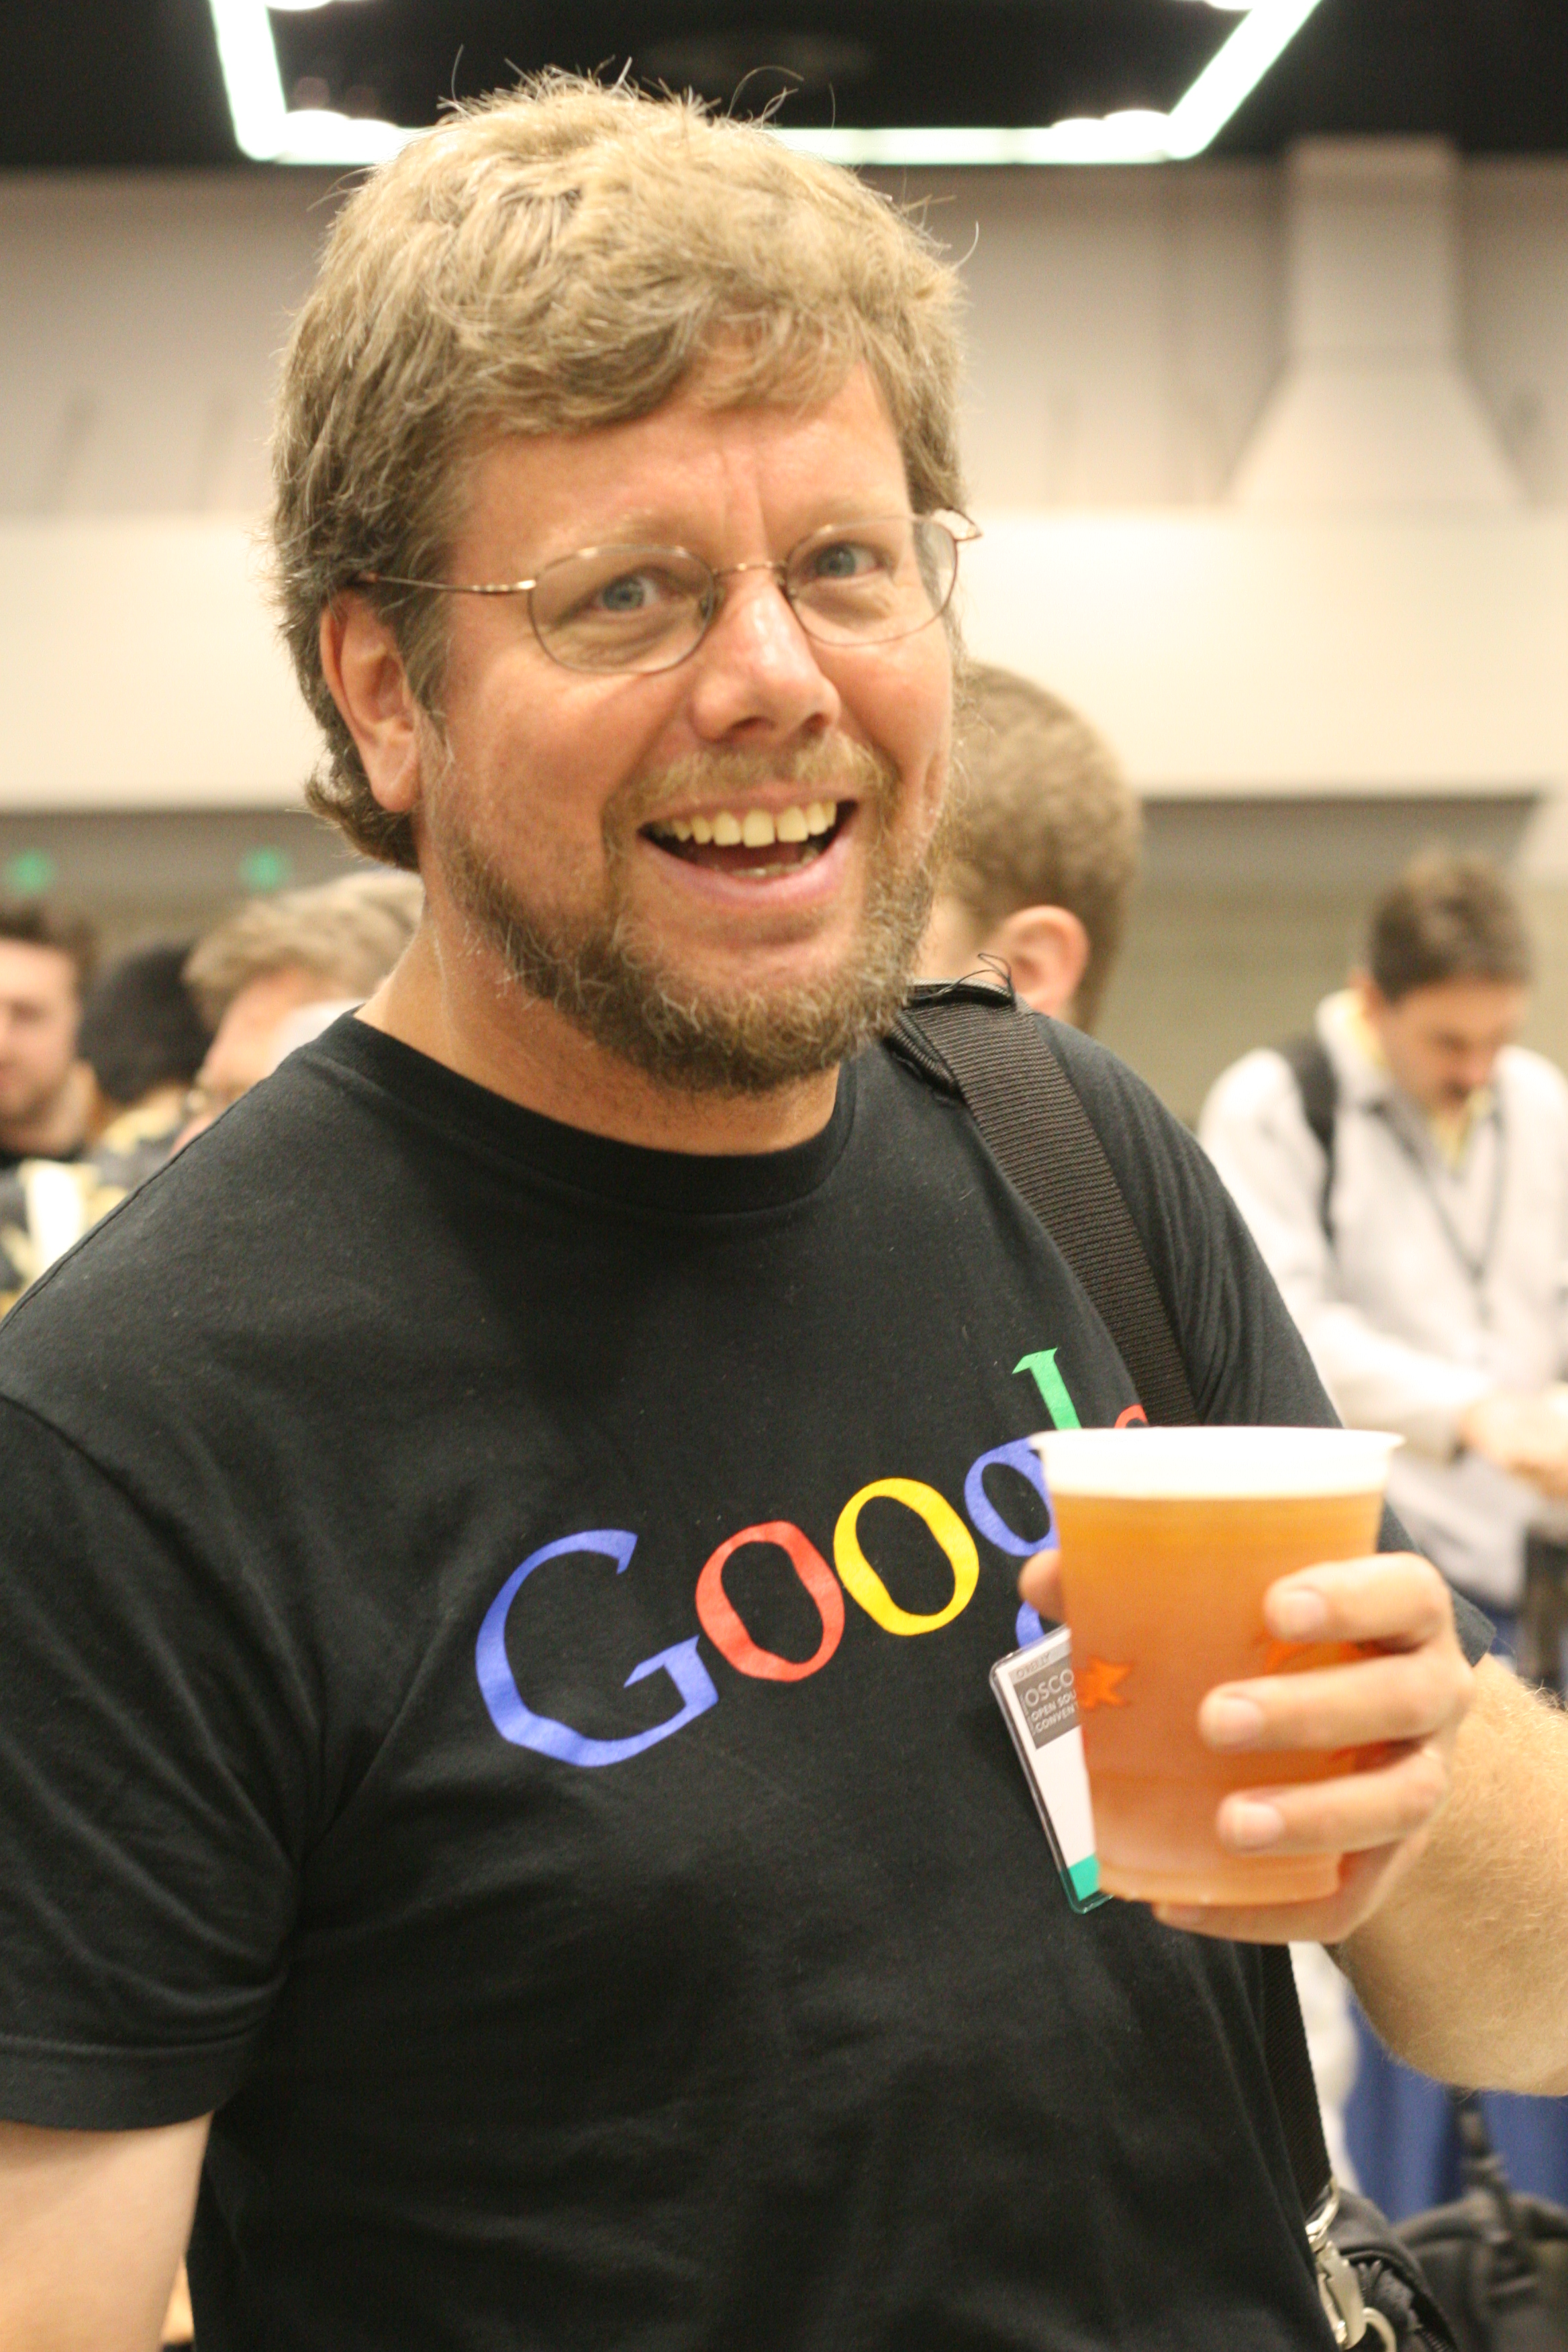
\includegraphics[keepaspectratio,height=0.8\textheight,width=\columnwidth]{Guido_van_Rossum_OSCON_2006}
            \caption{``Benevolent Dictator For Life''}
        \end{figure}
    \end{column}
    \end{columns}
\end{frame}

\begin{frame}{What is Python?}

Python is a modern, general-purpose, object-oriented, high-level language.

\begin{itemize}
    \item \emph{clean and simple language}: Easy to read and easy to learn syntax
    \item \emph{expressive language}: Fewer lines of code = fewer mistakes
    \item \emph{dynamically typed}: no need to define variable types or function arguments
    \item \emph{automatic memory management}: no need to allocate/deallocate memory
    \item \emph{interpreted}: No need to compile! Fast and easy
\end{itemize}

\end{frame}

\begin{frame}{Why Python?}
    \begin{columns}
    \begin{column}{0.5\textwidth}
    \begin{itemize}
        \item Free - free as in beer \Emph{AND} free as in speech
        \item General purpose - packages/modules for everything!
        \item Dynamic - no compiling
        \item Easy to read - enforces good structure!
        \item Open - everything is an object
    \end{itemize}
    \begin{block}{}
        It's harder to read code than to write it!
    \end{block}
    \end{column}
    \begin{column}{0.5\textwidth}
        \begin{figure}
            \centering
            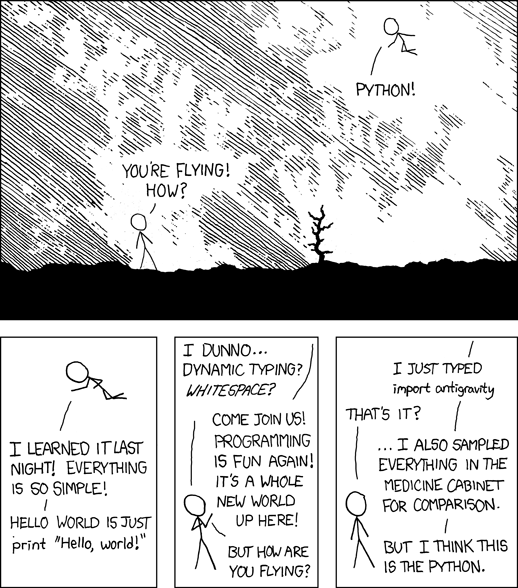
\includegraphics[width=\columnwidth,height=0.8\textheight,keepaspectratio]{figures/python.png}
        \end{figure}
    \end{column}
    \end{columns}
\end{frame}

\begin{frame}{Python vs. Matlab}
\begin{columns}[t]
\begin{column}{0.5\textwidth}
Disadvantages:
    \begin{itemize}
        \item Matlab is a commerical product - entire computing enviornment with code, IDE
        \item Matlab is expensive - Between \$49 - \$2150 per license! Extra for toolboxes
        \item Matlab is proprietary - Cannot inpect source code and restrictions on sharing 
        \item Matlab is closed - difficult to extend functionality 
    \end{itemize}
\end{column}
\pause
\begin{column}{0.5\textwidth}
    Advantages:
    \begin{itemize}
        \item Matlab handles arrays automatically and by design
        \item Lots of functionality - control design, linear algebra, optimization, ODEs etc.
        \item Real engineers (with funding) use it so students have to as well
        \item Simulink is still unmatched
        \item Powerful plotting capability
    \end{itemize}
\end{column}
\end{columns}

\begin{alertblock}{}
    \centering
    Python can offer all of the same functionality and some extra!
\end{alertblock}
\end{frame}

{\footnotesize
\begin{frame}{Python Philosophy - 20 aphorisms from the BDFL}

\begin{columns}[t]
\begin{column}{0.5\textwidth}
\begin{itemize}
    \item Beautiful is better than ugly.
    \item Explicit is better than implicit.
    \item \Emph{Simple is better than complex.}
    \item Complex is better than complicated.
    \item Flat is better than nested.
    \item Sparse is better than dense.
    \item Readability counts.
    \item Special cases aren't special enough to break the rules.
    \item Although practicality beats purity.
    \item Errors should never pass silently.
    \item Unless explicitly silenced.
\end{itemize}
\pause
\begin{block}{}
    \centering
    \texttt{>>> import this}
\end{block}
\end{column}
\begin{column}{0.5\textwidth}
    \begin{itemize}
        \item In the face of ambiguity, refuse the temptation to guess.
        \item \Emph{There should be one-- and preferably only one --obvious way to do it.}
        \item Although that way may not be obvious at first unless you're Dutch.
        \item Now is better than never.
        \item Although never is often better than \emph{right} now.
        \item If the implementation is hard to explain, it's a bad idea.
        \item If the implementation is easy to explain, it may be a good idea.
        \item Namespaces are one honking great idea -- let's do more of those!
    \end{itemize}
\end{column}
\end{columns}
\end{frame}
}

\end{document}

